\chapter{INVESTING AND TRADING}
\label{ch:investing}

This section covers the basics of two strategies - investing and trading - which you can deploy to help you reach your goals. Investing and trading are two very different methods of attempting to profit in the financial markets. With trading and investing, it is more about odds and probabilities than it is about certainties. You can drastically improve those odds by performing your own research (DYOR). As such, you should always dedicate some time and effort before making important decisions. Invest only in projects which you have identified as having potential or trade solely based on proper technical analysis or other research efforts.\medskip

Investing is the act of owning something, it could be an individual stock, a mutual fund, a property, or anything else you feel has less value today than you think it will have in the future. Trading is the actual transaction that occurs when you buy or sell investments. If you are an investor, typically it means you are a person who is holding on to something to earn a profit when the value increases. If you are a trader, then you are the person creating transactions. You are buying or selling the investments for yourself or others.

Traders attempt to take advantage of short term market swings, while investors take a more long term approach. Both investors and traders seek profits through market participation. In general, investors seek more substantial returns over an extended period through buying and holding. Traders, by contrast, take advantage of both rising and falling markets to enter and exit positions over a shorter time frame, making smaller, more frequent profits.

\begin{figure}
    \centering
    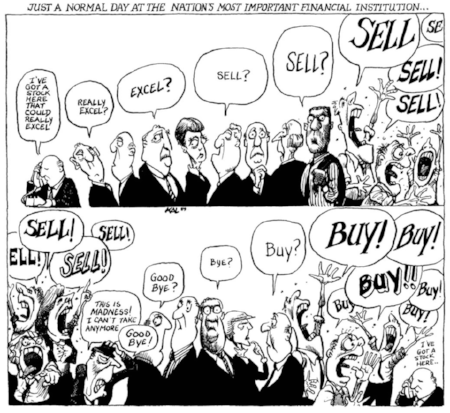
\includegraphics[width=.6\textwidth]{img/ch-investing/FOMOFUD.png}
    \caption{Fear, Uncertainty, and Doubt (FUD) evolves into Fear Of Missing Out (FOMO)}
    \label{fig:FOMOFUD}
\end{figure}

\section{Disclaimer}
The cryptomanual is the beginning of a journey, not the end. Where we present stimulating reading material we base on multiple years of research and experience, the results should only be treated as candidates for your own (further) research, not as a buy list or set of recommendations. Screening may help narrow a search based on pre-defined criteria, but it is not a substitute for independent research reflecting your criteria for investing/trading. Where we offer our readers evaluation tools, these are solely for informational and educational purposes so that readers are equipped with the basic tools required to perform their own (e)valuations. Our content is simply a starting point based on global assumptions that we have applied across the entire market - users should amend them as they deem fit and not regard them as a substitute for their own judgment.

\section{Economic Cycles}
Economic cycles or trade cycles are also known as business cycles. Solid (long-term) investment strategy should include and take into account the current position in the business cycle. 

    \medskip
    \tcbset{colback=orange!3!white,fonttitle=\bfseries}
    \begin{tcolorbox}
    [enhanced,
    title=Economic cycles explained,
    frame style=
    {left color=orange!85!black,right color=yellow!95!black}]
        \textit{\say{The economic cycle is the natural fluctuation of the economy between periods of expansion (growth) and contraction (recession). Factors such as gross domestic product (GDP), interest rates, levels of employment and consumer spending can help determine the current stage of the economic cycle. During times of expansion, investors seek to purchase companies in technology, capital goods, and primary energy sources. During times of contraction, investors look to buy shares of utility, financial and healthcare companies.} \footnote{Investopedia; \href{https://www.investopedia.com/terms/e/economic-cycle.asp}{What is the Economic Cycle}.}}
    \end{tcolorbox}

       
\subsection{Business cycles}
Business cycles represent the rise and fall in production output of goods and services in an economy. Business cycles are fluctuations in economic activity within that economy, which it experiences over many years or decades. These fluctuations include output from all sectors, including households, non-profits (NGOs), governments as well as other business outputs. Periods of economic expansion and contraction characterize the business cycle. During an expansion, the economy experiences growth, while a contraction (recession) represents a period of economic downturn or decline. \Cref{fig:economiccycle1,fig:economiccycle2} show the typical stages of the business cycle: expansion, peak, recession or contraction, depression, trough, and recovery.
Some economists believe that the business cycle is a natural part of the economy. Others believe that central banks indirectly control and influence the cycle by intervening with monetary policy.



\begin{figure}
    \begin{minipage}{.5\textwidth}
        \centering
        \subcaption{cycle excluding growth trend}
        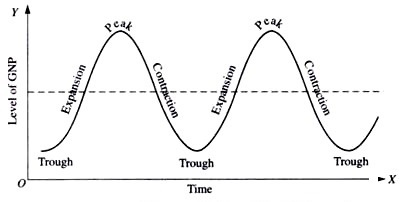
\includegraphics[width=\textwidth]{img/ch-investing/economic_cycle.jpg}
        \label{fig:economiccycle1}
    \end{minipage}
    \hfill
    \begin{minipage}{.5\textwidth}
        \centering
        \subcaption{cycle including growth trend}
        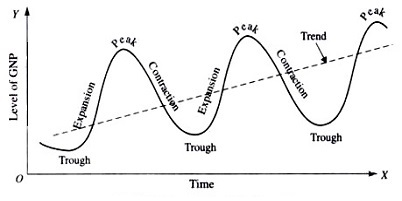
\includegraphics[width=\textwidth]{img/ch-investing/economic_cycletrend.jpg}
        \label{fig:economiccycle2}
    \end{minipage}  
    \label{fig:1-2}
  
    \caption{Business cycle excluding and including a generic growth trend}
    \source{Your Article Library; \href{http://www.yourarticlelibrary.com/macro-economics/theories-macro-economics/business-cycles-meaning-phases-features-and-theories-of-business-cycle/38063}{Knowledge Sharing Platform}.}
\end{figure}


\subsection{Credit cycles driving business cycles}
The credit cycle embodies the expansion and contraction and represents access to credit over time. It describes recurring phases of easy and tight borrowing and lending within the economy. Some economists, including Hyman Minsky and Steve Keen, regard credit cycles as the fundamental process driving the business cycle.
A credit cycle describes the phases of access to credit by borrowers. Credit cycles first go through periods in which funds are relatively easy to borrow; lower interest rates characterize these periods, decreasing lending requirements and an increase in the amount of available credit, which stimulates a general expansion of economic activity. A contraction follows these periods in the availability of funds. During the contraction of the credit cycle, interest rates climb, and lending rules become more strict, meaning that less credit is available for business loans, home loans, and other loans. The contraction period naturally continues until risks are reduced for the lending institutions, at which point the cycle troughs out and eventually starts over with renewed credit.


\section{Investing Versus Trading}
\label{sec:investingvstrading}

We tend to focus more on long term investing and wealth preservation; then we do on short term trading. Mainly originating from the fact that real value is created over a more extended period, and you can see your investments grow and develop. On top of this, trading effectively requires a lot of time, patience and effort to learn. Trading is usually not based on the fundamentals and principles of a particular cryptocurrency but based upon technical analysis of (historical) market movements, trends and price action. Trading usually involves much stress and is generally very time consuming since you're always on the clock, watching and analysing charts. Because of the technical nature of trading, you might easily overlook the intrinsic or fundamental value of a cryptocurrency or blockchain-based company or project.\medskip

With investing, this process is a little different. The fundamentals of a company or project are most important. Items such as the official whitepaper, the roadmap, community size, activeness and development are often leading. If you feel a project has a solid value proposition, it is usually related to the long term investment since many - if not all - plans are still in their infancy. For example, we could decide we want to invest in a company, which is designing a much-needed application to revolutionize voting. In itself, this has immense value, but the process of adopting this technology and implementing it in everyday life is long and tiring. You might monitor this project for a while, and if and when you are convinced it has potential and is moving in the right direction, you might decide to invest and start looking at the charts and price action. Then you analyze an optimal point of entry and determine if you feel comfortable taking a small position, after which you can expand periodically if so desired.\medskip

Here, the differences between the trading and investing approaches come into play. Traders might have bought this asset without having any personal connection with the actual product or service - they are just looking at positions with profit margins, regardless of the aim of the project itself. Therefore, they don't need to look at fundamentals since they can take advantage of fluctuating price action in minutes, hours or days. Investors feel comfortable with their investment and can ride out the storm (if there is any) where traders might sell to take fewer profits in much shorter periods. 

\begin{figure}
    \centering
    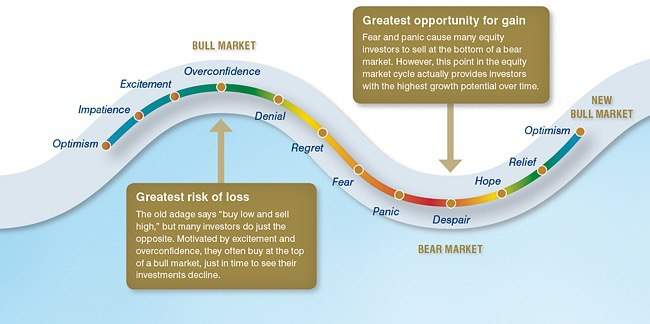
\includegraphics[width=.95\textwidth]{img/ch-investing/bear_bullmarket.jpg}
    \caption[Bear and bull markets and market psychology]{Market psychology is essentially what drives the so called \say{bear} and \say{bull} markets. In every stage of the emotional cycle there are decisions to be made by investors.}
    \label{fig:bear_bullmarket}
    \source{Brightscope; \href{https://www.brightscope.com/financial-planning/advice/article/30367/Breaking-The-Emotional-Cycle-Of-Investing}{Research and Data}.}
\end{figure}

\section{Investing}
The goal of investing is to gradually build wealth over an extended period through the buying and holding of a portfolio of stocks, baskets of stocks, mutual funds, bonds and other investment instruments. Investors often enhance their profits through compounding or reinvesting any profits and dividends into additional shares of stock. Investors often hold investments for years, or even decades, taking advantage of perks like (compounded) interest, dividends and stock splits along the way.\medskip

While markets inevitably fluctuate, investors will "ride out" the downtrends with the expectation that prices will rebound and any losses you suffered will eventually recover. Investors are typically more concerned with market fundamentals, such as price/earnings ratios and management forecasts.

    \medskip
    \tcbset{colback=orange!3!white,fonttitle=\bfseries}
    \begin{tcolorbox}
    [enhanced,
    title=Investors,
    frame style=
    {left color=orange!85!black,right color=yellow!95!black}]
            \textit{Investors speculate on the development of the cryptocurrency application and its eventual adoption, which will bring about a premium over its current prices. He or she minimizes risks by doing due diligence, diversification, and portfolio management.}
    \end{tcolorbox}
    \medskip

\noindent As a rule of thumb, when investing, ask yourself the following question; do I want and need this and if so, how badly? Do I want to use this utility in the future and is it beneficial to other people and me?\medskip

When you conclude that you feel safe with this investment, you can start looking at the optimal entry points (this is the same for both short and long term) on a platform such as \href{https://www.coinigy.com/?r=17fa0d35}{Coinigy} or \href{https://www.tradingview.com/}{TradingView}. The following highlights might be of importance:\medskip  

\begin{enumerate}
    \setlength\itemsep{0em}
    \item Technical analysis - entry and exit points $\longrightarrow$ buy low, sell high %\cref{sec:technicalanalysis}
    \item Accumulation, periodic buys and dollar-cost averaging (same amount in US\$ or any other currency)
    \item Don't be afraid to take profits! FOMO can lead to your emotions taking over
    \item Learn to recognize your emotions and how they influence your decision making
    \item Learn about your trading tools, i.e. use stop losses if so desired
    \item Give your investments time to mature - try to imagine what your investment could be worth years from now
    \item Periodically re-assess your situation and decide if you keep your position(s) or perhaps need to diversify, re-balance or buy/sell
\end{enumerate}

\section{Trading}
Trading, on the other hand, involves the more frequent buying and selling of stock, commodities, currency pairs or other instruments such as cryptocurrencies, to generate returns that outperform buy-and-hold investing as mentioned above. While investors may be content with a 10\% to 15\% annual return, traders might seek a 10\% return each month.\medskip

    \medskip
    \tcbset{colback=orange!3!white,fonttitle=\bfseries}
    \begin{tcolorbox}
    [enhanced,
    title=Traders,
    frame style=
    {left color=orange!85!black,right color=yellow!95!black}]
        \textit{Traders speculate a specific direction of the prices based on historical data and patterns. In doing so, they minimize risk with a set of technical tools and expertise. Trading can be highly stressful, but traders may profit from both bear and bull markets at the cost of the considerable higher risk involved.}
    \end{tcolorbox}
    \medskip

Trading profits are generated by buying at a lower price and selling at a higher price within a relatively short period. The reverse is also true: trading profits are made by selling at a higher price and buying to cover at a lower price (known as selling short) to profit in falling markets. Where buy-and-hold investors wait out less profitable positions, traders must make profits (or take losses) within a specified period, and often use a protective stop-loss order to close out losing positions at a predetermined price level automatically. Traders often employ technical analysis tools, such as moving averages and stochastic oscillators, to find high-probability trading setups.

\subsection{Trading styles}
In trading, several styles refer to the time-frame or holding period in which cryptocurrencies, stocks, commodities or other trading instruments are bought and sold. Traders generally fall into one of the four categories presented in \cref{tab:tradertypes}. Traders often choose their trading style based on factors including account size, amount of time that they can dedicate to trading, level of trading experience, personality and risk tolerance (high risk/reward ratio exposure).

\begin{table}[!htb]
\centering
\caption{Trading styles}
\begin{tabular}{ll}
\toprule
\textbf{Trader type}         &   \textbf{Positions held}                 \\
\midrule
                   
Position          &    from months to years (might also be called investing)                 \\
Swing             &    from days to weeks                    \\
Day               &    throughout the day only - no overnight positions\\
Scalp             &    for seconds to minutes with no overnight positions \\
\bottomrule                                     
\label{tab:tradertypes}
\end{tabular}
\end{table}

\subsection{Your emotions will impact your decision making}
Whatever you want to buy, it will still be there tomorrow, and perhaps it will be even cheaper. Be aware of the following at all times and try not to let certain emotions impact your decision-making capabilities:

\begin{enumerate}
    \item When markets move, so does overall market sentiment. People get excited and are prone to overextend. Don't overextend. Recognize hype and learn to take profits or risk losing it all.
    \item Do not become emotionally attached to your investment - you will not get every trade right; do not take it personally. Always aim for rational choices, but if you're aiming at the long term, keep your investment choices in line with your personal beliefs.
    \item Do not get scammed. People may have their reasons for steering you in any particular direction. Your level of due diligence is directly related to your ability to recognize and identify a potential red flag.
    \item Do not panic or give in to hype (FOMO - FUD). Rationally think about your decisions, based on your analysis, which is further substantiated by your research.
\end{enumerate}

\section{3 Technical Trading Indicators for starters}
\begin{enumerate}
    \item RSI
    \item STOCH
    \item MACD
\end{enumerate}



\section{Entry and Exit Strategies}
\begin{enumerate}
    \item Stop Loss
    \item Dollar cost average
    \item 
\end{enumerate}
